\documentclass[tikz,border=10pt]{standalone}
\usepackage{mathabx}
\usetikzlibrary{backgrounds}
\usepackage{newunicodechar}
\newunicodechar{♮}{$\natural$}
\newunicodechar{♭}{$\flat$}
\newunicodechar{♯}{$\sharp$}
\newunicodechar{➚}{$\nearrow$}
\newunicodechar{➘}{$\searrow$}
\newunicodechar{Ȧ}{\stackon[0.8pt]{A}{.}}
\newunicodechar{Ḃ}{\stackon[0.8pt]{B}{.}}
\newunicodechar{Ċ}{\stackon[0.8pt]{C}{.}}
\newunicodechar{Ḋ}{\stackon[0.8pt]{D}{.}}
\newunicodechar{Ė}{\stackon[0.8pt]{E}{.}}
\newunicodechar{Ḟ}{\stackon[0.8pt]{F}{.}}
\newunicodechar{Ġ}{\stackon[0.8pt]{G}{.}}


\def\centerarc[#1](#2)(#3:#4:#5);%
{
  \draw[#1]([shift=(#3:#5)]#2) arc (#3:#4:#5);
}


\begin{document}
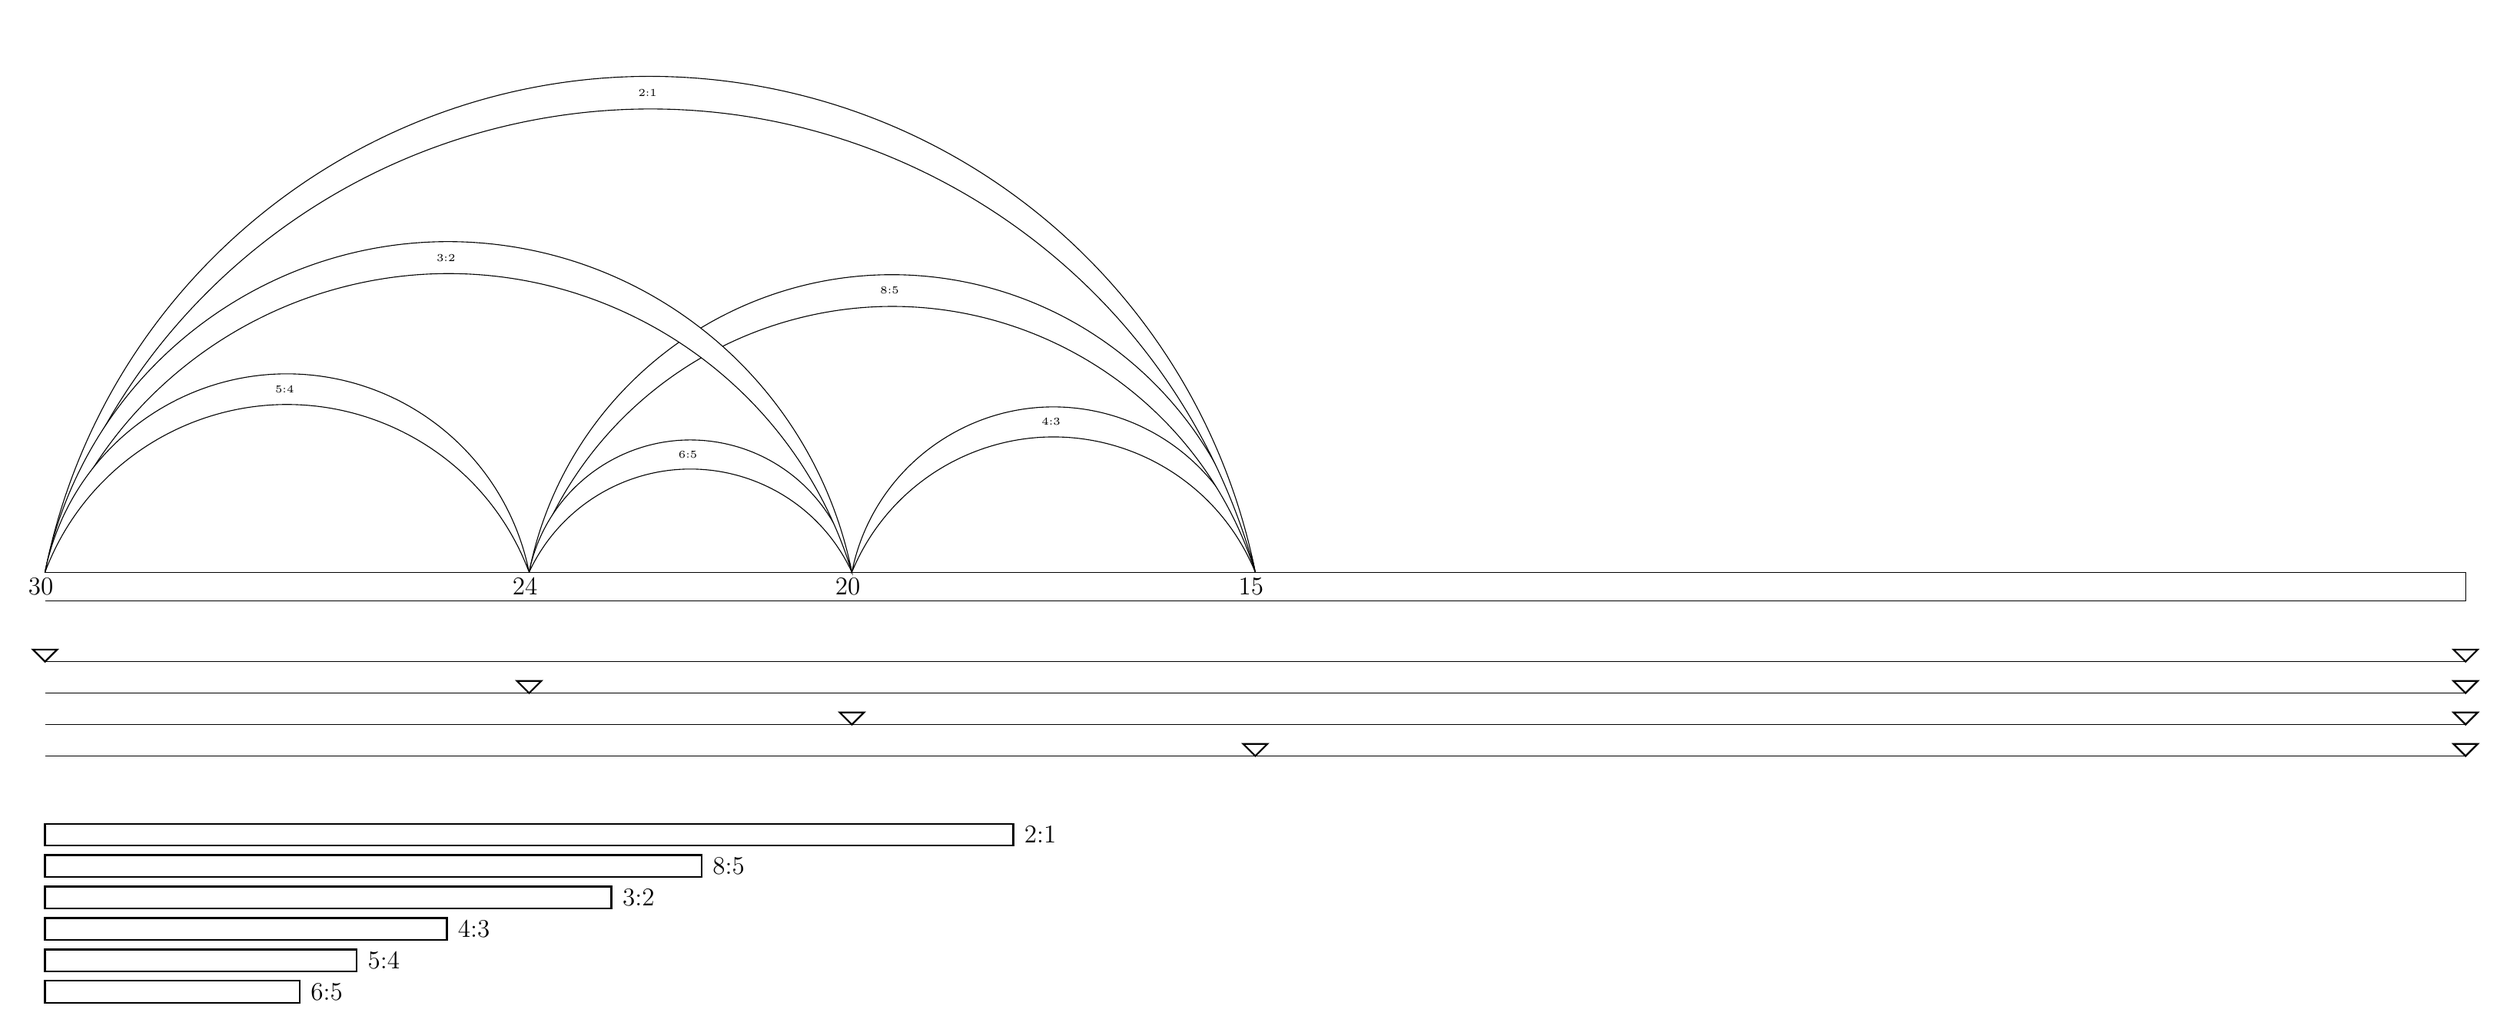
\begin{tikzpicture}

\draw (0.0,0.0) -- (40.0,0.0);
\draw (0.0,-0.48000002) -- (40.0,-0.48000002);
\draw (40.0,-0.48000002) -- (40.0,0.0);
\draw[fill=white] (13.333333,0.0) arc[start angle=168.69004417272032, end angle=11.309931807932047, radius=3.3993466] arc[start angle=22.293628167894898, end angle=157.7063631806831, radius=3.6026227] -- cycle;
\node[align=center] at (16.666666,2.484318) { \tiny 4:3 };
\draw[fill=white] (8.0,0.0) arc[start angle=168.69007234725063, end angle=11.309932661705695, radius=6.1188235] arc[start angle=17.57125928141018, end angle=162.42872523697866, radius=6.293648] -- cycle;
\node[align=center] at (14.0,4.6562357) { \tiny 8:5 };
\draw[fill=white] (8.0,0.0) arc[start angle=168.69007234725063, end angle=11.309932661705695, radius=2.719477] arc[start angle=24.820543736253033, end angle=155.1794578576087, radius=2.938064] -- cycle;
\node[align=center] at (10.666666,1.9454372) { \tiny 6:5 };
\draw[fill=white] (0.0,0.0) arc[start angle=168.69007234725063, end angle=11.309932661705695, radius=10.198039] arc[start angle=15.10957543472025, end angle=164.89041932895233, radius=10.3580885] -- cycle;
\node[align=center] at (10.0,7.928064) { \tiny 2:1 };
\draw[fill=white] (0.0,0.0) arc[start angle=168.69004502649395, end angle=11.309932661705695, radius=6.7986927] arc[start angle=16.96170587912156, end angle=163.0382922996456, radius=6.969856] -- cycle;
\node[align=center] at (6.6666665,5.200941) { \tiny 3:2 };
\draw[fill=white] (0.0,0.0) arc[start angle=168.6900732010243, end angle=11.30993351547934, radius=4.0792155] arc[start angle=20.55604511851658, end angle=159.44395306025058, radius=4.2720017] -- cycle;
\node[align=center] at (4.0,3.0256085) { \tiny 5:4 };
\node[align=center] at (0.0, -0.24000001) { \large 30 };
\node[align=center] at (8.0, -0.24000001) { \large 24 };
\node[align=center] at (13.333333, -0.24000001) { \large 20 };
\node[align=center] at (20.0, -0.24000001) { \large 15 };
\draw (0.0,-1.48) -- (40.0,-1.48);
\draw[thick] (0.0, -1.48) -- (0.2, -1.2800001) -- (-0.2, -1.2800001) --  cycle;
\draw[thick] (40.0, -1.48) -- (40.2, -1.2800001) -- (39.8, -1.2800001) --  cycle;
\draw (0.0,-2.0) -- (40.0,-2.0);
\draw[thick] (8.0, -2.0) -- (8.2, -1.8000001) -- (7.8, -1.8000001) --  cycle;
\draw[thick] (40.0, -2.0) -- (40.2, -1.8000001) -- (39.8, -1.8000001) --  cycle;
\draw (0.0,-2.5200002) -- (40.0,-2.5200002);
\draw[thick] (13.333333, -2.5200002) -- (13.533333, -2.3200002) -- (13.133333, -2.3200002) --  cycle;
\draw[thick] (40.0, -2.5200002) -- (40.2, -2.3200002) -- (39.8, -2.3200002) --  cycle;
\draw (0.0,-3.04) -- (40.0,-3.04);
\draw[thick] (20.0, -3.04) -- (20.2, -2.84) -- (19.800001, -2.84) --  cycle;
\draw[thick] (40.0, -3.04) -- (40.2, -2.84) -- (39.8, -2.84) --  cycle;
\draw[thick] (0.0, -4.16) -- (15.999503, -4.16) -- (15.999503, -4.52) -- (0.0, -4.52) --  cycle;
\node[anchor=west] at (16.059504, -4.3399997) { \large 2:1 };
\draw[thick] (0.0, -4.68) -- (10.848815, -4.68) -- (10.848815, -5.04) -- (0.0, -5.04) --  cycle;
\node[anchor=west] at (10.908814, -4.86) { \large 8:5 };
\draw[thick] (0.0, -5.2000003) -- (9.35911, -5.2000003) -- (9.35911, -5.56) -- (0.0, -5.56) --  cycle;
\node[anchor=west] at (9.419109, -5.38) { \large 3:2 };
\draw[thick] (0.0, -5.72) -- (6.6403947, -5.72) -- (6.6403947, -6.0799994) -- (0.0, -6.0799994) --  cycle;
\node[anchor=west] at (6.7003946, -5.8999996) { \large 4:3 };
\draw[thick] (0.0, -6.24) -- (5.1506896, -6.24) -- (5.1506896, -6.6) -- (0.0, -6.6) --  cycle;
\node[anchor=west] at (5.2106895, -6.4199996) { \large 5:4 };
\draw[thick] (0.0, -6.7599998) -- (4.2084203, -6.7599998) -- (4.2084203, -7.12) -- (0.0, -7.12) --  cycle;
\node[anchor=west] at (4.26842, -6.94) { \large 6:5 };
\end{tikzpicture}
\end{document}